\documentclass[twoside]{article}

\usepackage[sc]{mathpazo}
\usepackage[T1]{fontenc}
\usepackage{microtype}
\usepackage{color}
\usepackage[twoside,height=24cm,left=3cm]{geometry}
\usepackage{multicol}
\usepackage[hang, small,labelfont=bf,up,textfont=it,up]{caption}
\usepackage{booktabs}
\usepackage{float}
\usepackage{hyperref}
\usepackage[spanish]{babel}
\usepackage[utf8]{inputenc}
\usepackage{graphicx}
\usepackage{amsmath}
\usepackage{amssymb}
\usepackage{enumerate}
\usepackage{bm}
\usepackage{lettrine}
\usepackage{paralist}
\usepackage{abstract}
\usepackage{titlesec}
\usepackage{fancyhdr}
\usepackage{fullpage}
\usepackage{booktabs}
\usepackage{tikz}
\usepackage{pgfplots}
\usepackage{float}
\usepackage{hyperref}
\usepackage{color}
\usepackage{graphicx}
\usepackage{xfrac}
\usepackage{titling}
\usepackage{multirow}
\usepackage{subcaption}
\usepackage{natbib}
\usepackage{siunitx}
\usepackage[format=plain,labelfont=it,textfont=it]{caption}
\usepackage{geometry}
\usepackage{multicol}

\renewcommand{\abstractnamefont}{\normalfont\bfseries}
\renewcommand{\abstracttextfont}{\normalfont\small\itshape}
\newcommand{\grad}{$^{\circ}$}

\linespread{1.05}
\setlength\parindent{0pt}
\setlength\columnsep{20pt}
\setlength{\headheight}{12.0pt}
\addto\captionsspanish{
    \def\contentsname{\'Indice}
    \def\bibname{Referencias}
    \def\tablename{Tabla}
    \def\abstractname{Resumen}
}
\pagestyle{fancy}
\fancyhead{}
\fancyfoot{}
\fancyhead[C]{Laboratorio 7 $\bullet$ Cátedra Ledesma}
\fancyfoot[RO,LE]{\thepage}
\hyphenpenalty=100000
\pgfplotsset{compat=1.10}
\geometry{left=15mm,right=15mm}

\begin{document}

\begin{titlepage}
\begin{center}

\textsc{\LARGE Laboratorio 7}\\[0.5cm]
\textsc{\Large Departamento de Física}\\[0.5cm]
\textsc{\Large Facultad de Ciencias Exactas y Naturales}\\[0.5cm]
\textsc{\Large Universidad de Buenos Aires}\\[1.5cm]

1er cuatrimestre 2021\\[1.5cm]

{ \huge \bfseries Aplicación del efecto Josephson a la generación de señales arbitrarias con aplicaciones a la metrología}\\[1.5cm]


%\begin{minipage}{0.8\textwidth}
%\begin{flushleft} \large


Alumno:
Pinto Zárate, José Daniel\\
\href{mailto:dann.2207@gmail.com}{dann.2207@gmail.com}

%\end{flushleft}
%\end{minipage}
\vfill
{\large \today}
\end{center}
\end{titlepage}

\begin{abstract}

En este trabajo se armó e implementó un sistema Josephson pulsado (JAWS)

\end{abstract}

\begin{multicols}{2}

\section{Introducción}

El JAWS (Josephson Arbitrary Waveform Synthesizer), o sistema Josephson pulsado, es un sistema utilizado para la generación de señales de tensión de forma arbitraria basado en el efecto Josephson, en el cual la tensión generada depende de constantes fundamentales. Pertenece a la familia de sintetizadores basados en el efecto Josephson, como el sistema Josephson programable (PJVS) y el sistema Josephson convencional (CJVS). En la figura \ref{fig:intro_mapaMundoJosephson} se muestra un mapa esquemático que muestra algunos de estos proyectos que se están llevando a cabo actualmente en diferentes centros.
% mencionar el reciente cambio del sistema de unidades
\begin{figure}[H]
    \centering
    \includegraphics[width=\linewidth]{figuras/intro/mapaMundoJosephson.jpg}
    \caption{Mapa esquemático de los actuales proyectos de sistemas de sintetización de señales basados en el efecto Josephson}
    \label{fig:intro_mapaMundoJosephson}
\end{figure}

Una de las ventajas principales del JAWS es que posibilita la minimización del ruido de la señal generada, y para esto se utiliza un método de modulación de pulsos llamado Sigma-Delta ($\Sigma-\Delta$). Esta modulación se usa no solo en metrología, como en nuestro caso, sino también en 

El JAWS tiene varias ventajas como generador de señales, ya que genera una tensión que tiene dependencia total en constantes universales, y tiene trazabilidad a las mismas especificadas por la ecuación de Josephson para el JAWS \ref{eq:intro_ecuacionJosepshon} \cite{behr2012}.

\begin{equation}
    V = A_{\Sigma\Delta} \Phi_0 f n M
    \label{eq:intro_ecuacionJosephson}
\end{equation}

donde $M$ es la cantidad de junturas del array

    \subsection{Efecto Josephson y su aplicacion en el JAWS}

    El efecto Josephson es un fenómeno que se presenta en las junturas superconductoras, como la que se muestra en la figura \ref{fig:intro_junturaJosephson}, cuando a estas se las somete a diferentes señales de corriente variable. Hay varias manifestaciones de este efecto, siendo las mas conocidas las del efecto Josephson AC y DC; en el JAWS se trabaja con este efecto utilizando trenes de pulsos de corriente a altas frecuencias, del orden de las microondas, generando un efecto similar al del efecto Josephson AC, con la diferencia de que se utilizan pulsos en vez de una señal contínua, que es cuando se envía un tren de pulsos de microondas a un array de junturas Josephson en serie. Otros efectos relacionados son el efecto Josephson AC, que es cuando . Dichos efectos estan entre los que se utilizan para construir otros sintetizadores que aprovechan el mismo fenómeno, como el sistema Josephson programable (PJVS), o el convencional (CJVS). 

    El efecto josephson pulsado consiste en una conversión entre una señal de tren de pulsos AC,  y 



\begin{figure}[H]
    \centering
    \includegraphics[width=\linewidth]{figuras/intro/junturaJosephson.png}
    \caption{Efecto Josephson en una juntura superconductora}
    \label{fig:intro_junturaJosephson}
\end{figure}

La curva I-V o curva característica es el gráfico de la tensión en función de la corriente, y en una juntura superconductora se cumple que, en el régimen de temperaturas bajas en las que hay superconducción, dicha curva se aplane, como se muestra en la figura XXX. 

[XXX: grafico de behr de la IV de 1 juntura]

Cuando se trata de varias junturas conectadas en serie, como en el array, este nivel de tensión en el que se aplana puede variar, 

Un plateau es una zona de la curva I-V en la que la tensión es constante en un rango contínuo de corrientes. Si la corriente que atraviesa el JAWS se mantiene dentro de una de estas zonas, se verifica la ecuación de Josephson.
La corriente de compensación se agrega para que el array se encuentre en un plateau, como se muestra en la figura \ref{fig:intro_plateau}. La señal debe estar en un plateau ya que es un requisito para que se verifique la ecuaciónde Josephson.

Si el sistema se encuentra en un plateau, se cuantiza el área de la curva de corriente vs tiempo, de modo que aunque los pulsos se deformen, siempre que mantengan su área, se obtendrán los mismos resultados \cite{benz1998}. 

La cantidad de plateaus es del orden de la cantidad de junturas del array. %no estoy seguro

El cambio de temperatura es un factor que puede alterar la forma de estos pulsos, y una posible fuente de error. Si por ejemplo los pulsos se ensanchan hasta unirse, se podría perder información de la señal en las zonas en las que haya alta densidad de pulsos.



\begin{figure}[H]
    \centering
    \includegraphics[width=\linewidth]{figuras/intro/plateau.png}
    \caption{Señal corrida a la derecha del plateau}
    \label{fig:intro_plateau}
\end{figure}

\section{Descripción de la simulación numérica}

La generación de los trenes de pulsos utlizados fue hecha usando el algoritmo de modulación Sigma-Delta standard de primer orden. Este es un método iterativo basado en el esquema de bloques de la figura \ref{fig:numerica_esquemaBloques1erOrden}. La implementación se basó en los trabajos de Aziz \cite{aziz1996} y De la Rosa \cite{delarosa2011}. Existen implementaciones de este método pero que tienen un enfoque distinto, como la libreria de Python de G. Venturini \cite{DSpython} y la librería de MATLAB de R. Schreier \cite{DSmatlab}.

\begin{figure}[H]
    \centering
    \includegraphics[width=\linewidth]{figuras/numerica/esquemaBloques1erOrden.png}
    \caption{Diagrama de bloques correspondiente a la modulación $\Sigma\Delta$ de 1er orden}
    \label{fig:numerica_esquemaBloques1erOrden}
\end{figure}

%En este trabajo se implementó, siguiendo diferentes publicaciones (\cite{delarosa2011}, \cite{aziz1996}), el algoritmo de modulación Sigma-Delta de 1er orden en Python. Esto permitió explorar diferentes aspectos del método que no eran muy accesibles desde otras implementaciones, de manera muy sencilla.
%Las implementaciones anteriores contienen optimizaciones adicionales que por el momento nuestro código no incluye. La más conocida es el paquete de Matlab de Richard Scherier \cite{DSmatlab}, sobre la cual se basa el paquete de Python de G. Venturini \cite{DSpython}.

%El código utilizado genera distintas variables presentes en la modulación sigma delta, y permite hacer un análisis muy detallado a partir de las mismas. 
En la figura \ref{fig:bloques} se muestra el diagrama de bloques representativo del algoritmo de modulación de 1er orden \cite{script}.

\begin{figure}[H]
\centering
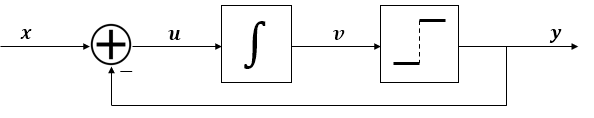
\includegraphics[width=\linewidth]{figuras/bloques_1erorden.png}
\caption{Diagrama de bloques correspondiente a la modulación $\Sigma\Delta$ de 1er orden}
\label{fig:bloques}
\end{figure}

En el apéndice se describe muy brevemente como se leen estos diagramas, y como se pueden traducir a un método iterativo en las 4 variables presentes: $x,u,v,y$.
La primera, $x$, representa la señal analógica de entrada, que es la señal que queremos generar. $u$ y $v$ son variables auxiliares, en donde $v$ es la integral de $u$, y $u$ es la diferencia $x-y$. $y$ es la salida final del cuantizador, que tiene en nuestro caso solo 2 valores posibles.



En la figura \ref{fig:integrador} se muestra mejor el comportamiento de las variables $u$ y $v$ para cuando se quiere generar una señal DC de valor 0.8 u.a. Se observa que hay un período en el que la señal $u=x-y$ es ligeramente negativa, esto es porque $x=0.8$ es ligeramente inferior al nivel superior $y=1$ (todo en unidades arbitrarias). Durante este período, se van sumando estos valores de $u$ al valor de $v$, que en la figura \ref{fig:integrador} es la pendiente negativa que está en el área de integración negativa, sombreada en azul.


\begin{figure}[H]
\centering
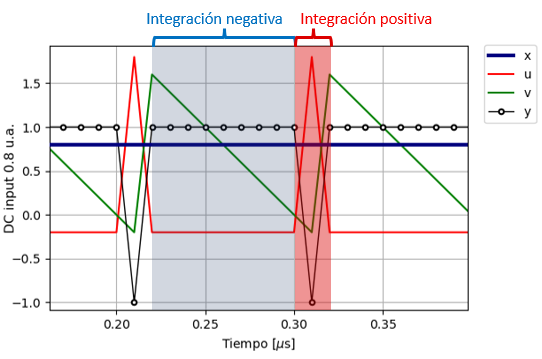
\includegraphics[width=\linewidth]{figuras/integracion.png}
\caption{Ejemplo del funcionamiento del integrador en la modulación a 1er orden}
\label{fig:integrador}
\end{figure}

Llega un punto en que $v$ pasa a ser negativo, de modo que, al pasar al cuantizador, generará un pulso $y$ negativo, luego de varios positivos. Esto es lo que se ve en el área de integración positiva: el valor de $u$, en ese lapso muy corto de tiempo, es positivo y muy grande, de tal manera que basta solo uno para volver al régimen de pulsos positivos. De esta manera el algoritmo genera la proporción de pulsos negativos y positivos deseada.

\section{Descripción del experimento}

El esquema experimental del JAWS se muestra en la figura \ref{fig:experimental_1}. Se utilizó un generador de pulsos programable (FPGA) Xilinx Zynq-7000, que enviaba pulsos de corriente a una frecuencia de \SI{5}{\giga\hertz}. Dicho FPGA tiene tres patrones de calibración, que se usaron para calibrar los pulsos programados. Estos pulsos fueron enviados mediante un cable semirrígido, que soporta el rango de frecuencias utilizado en el experimento, y viajaban hacia el array sumergido en Helio líquido a \SI{4.2}{\kelvin}

\begin{figure}[H]
    \centering
    \includegraphics[width=0.75\linewidth]{figuras/experimental/1.png}
    \caption{Esquema del arreglo experimental para la prueba del JAWS}
    \label{fig:experimental_1}
\end{figure}

A la señal de pulsos de la FPGA se le agrega una corriente adicional de frecuencia \SI{3.125}{\kilo\hertz} mediante un generador de funciones (Tektronix AFG1062), dicha señal es la corriente de compensación.

En la figura \ref{fig:experimental_sumaDeCorrientes} \cite{kieler2007} se muestra un detalle de como se suman las señales de pulsos con la corriente de compensación. El chip JAWS tiene pines por los que entra dicha corriente, mientras que los pulsos entran a través de la entrada externa, mediante el cable semirrígido.

\begin{figure}[H]
    \centering
    \includegraphics[width=0.75\linewidth]{figuras/experimental/sumaDeCorrientes.png}
    \caption{Detalle de la suma de la corriente de compensación y el tren de pulsos de la FPGA}
    \label{fig:experimental_sumaDeCorrientes}
\end{figure}

De no estar presente la corriente de compensación, el ruido de la señal podría amplificarse incluso pasando por el array. En la figura XXX se muestra este efecto en un experimento del NIST, en el que se aprecia que cuando se encuentra en el plateau, el array reacciona bien disminuyendo el ruido como se espera.

\begin{figure}[H]
    \centering
    \includegraphics[width=0.75\linewidth]{figuras/experimental/conYSinPlateau.png}
    \caption{Comparación entre el nivel de ruido cuando el sistema se encuentra dentro y fuera de un plateau}
    \label{fig:experimental_conYSinPlateau}
\end{figure}

\section{Resultados y Análisis}

    \subsection{Simulación numérica}

    Usando nuestro script \cite{script}, generamos los pulsos correspondientes a una señal DC para reproducir los resultados que se muestran en \cite{aziz1996}. En la figura 

    \subsection{Pruebas experimentales con la FPGA}

    En la figura \ref{fig:resultados_patron32FPGA} se muestran las mediciones de la calibración de la FPGA. Se puede ver como se deforman los pulsos de corriente.

    \begin{figure}[H]
        \centering
        \includegraphics[width=0.75\linewidth]{figuras/resultados/patron32FPGA.png}
        \caption{Medición de la salida de la FPGA en el modo de patrón de 1 pulso cada 32}
        \label{fig:resultados_patron32FPGA}
    \end{figure}



\end{multicols}

%\newpage
\bibliographystyle{unsrt}
\bibliography{references.bib}


\nocite{*} % Insert publications even if they are not cited in the poster

\end{document}
